\section*{Espejos planos}

\item (*) Demuestre que la imagen dada por un espejo plano de una fuente puntual es, sin ninguna aproximación, otra fuente puntual, ubicada simétricamente respecto del plano del espejo.
Analice los casos que corresponden a objetos reales o virtuales.


\item ¿Cuál es la mínima longitud de un espejo plano vertical para que un hombre de \SI{1.8}{\metre} se vea entero?
¿Es importante conocer la distancia hombre-espejo? 


\item (*)
\begin{minipage}[t][1.5cm]{0.8\textwidth}
Realice un diagrama de rayos que le permita localizar las imágenes de la flecha que se muestra en la figura.
Para un punto de la flecha dibuje una porción del frente de ondas emergente y los correspondientes frentes reflejados.
\end{minipage}
\begin{minipage}[c][0.6cm][t]{0.1\textwidth}
	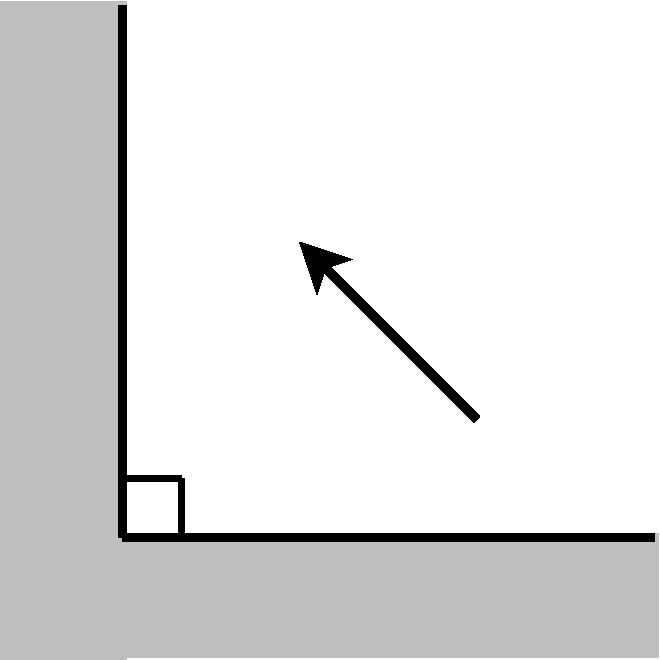
\includegraphics[width=\textwidth]{ej3-11}
\end{minipage}



\item
\begin{minipage}[t][0cm]{0.65\textwidth}
Dos espejos planos forman un ángulo $\alpha$ como lo indica la figura.
\end{minipage}
\begin{minipage}[c][1.5cm][t]{0.3\textwidth}
	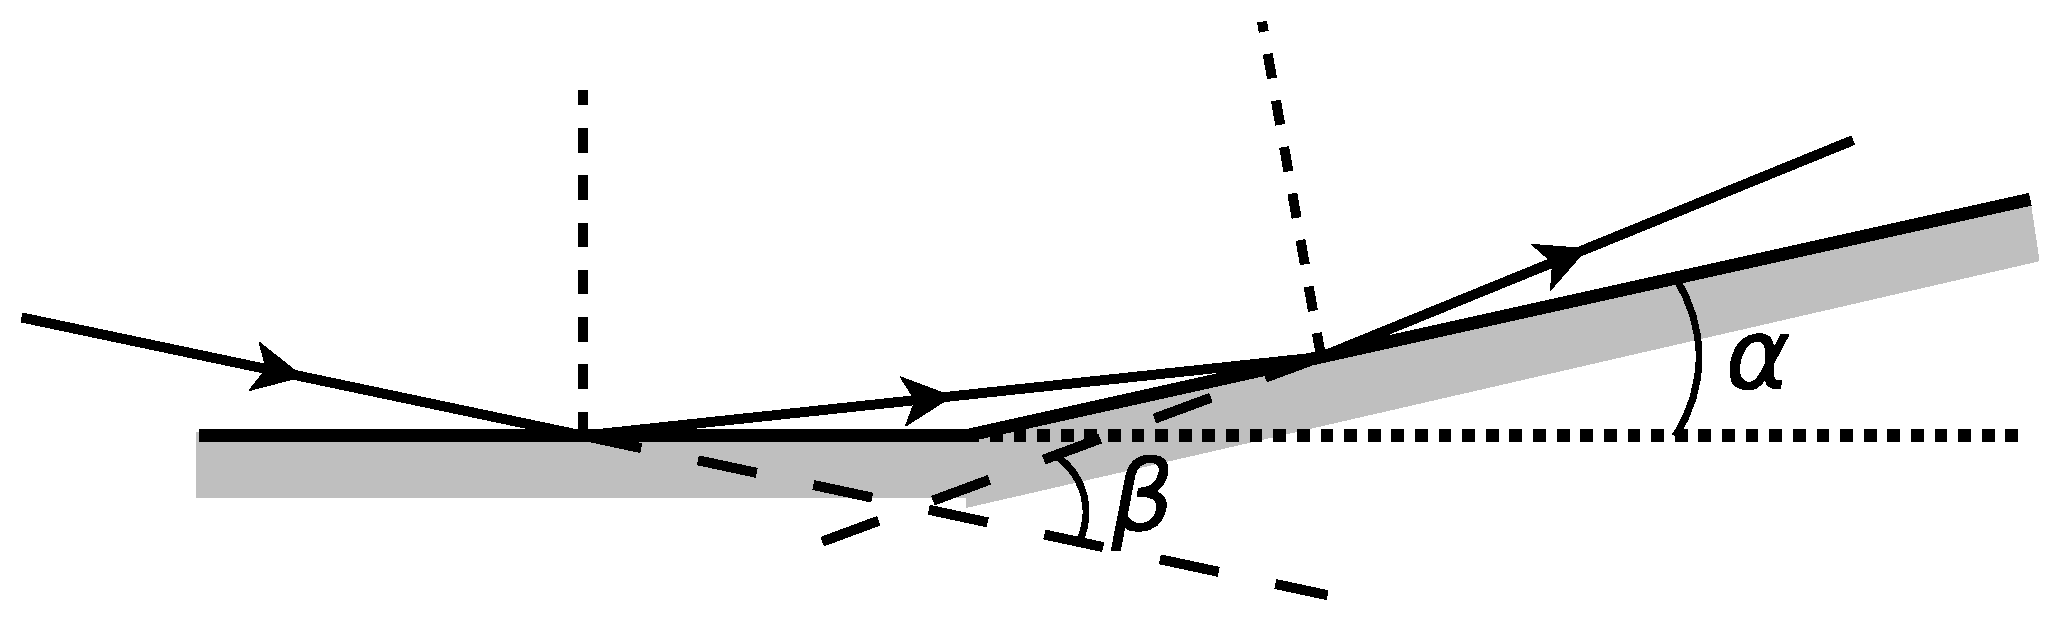
\includegraphics[width=\textwidth]{ej3-12}
\end{minipage}
\begin{enumerate}
	\item Un rayo de luz contenido en un plano perpendicular a la intersección de los espejos incide sobre uno de ellos, se refleja e incide en el otro (ver figura).
	Calcule el ángulo \(\beta\) que forman los rayos incidente y emergente.
	\item (*) Suponga la misma geometría que en a) pero ahora iluminada por una fuente puntual, demuestre que las imágenes se encuentran sobre una circunferencia con centro en el vértice de los espejos.
	En el caso en que la fuente está ubicada de tal modo que sólo se producen dos imágenes, y que el ángulo es muy pequeño, calcule la distancia entre ellas (espejos de Fresnel).
\end{enumerate}
